\documentclass{standalone}
\usepackage{tikz}
\usepackage{ctex,siunitx}
\setCJKmainfont{Noto Serif CJK SC}
\usepackage{tkz-euclide}
\usepackage{amsmath}
\usetikzlibrary{patterns, calc,3d}
\usetikzlibrary {decorations.pathmorphing,decorations.pathreplacing,decorations.shapes}
\begin{document}
\small
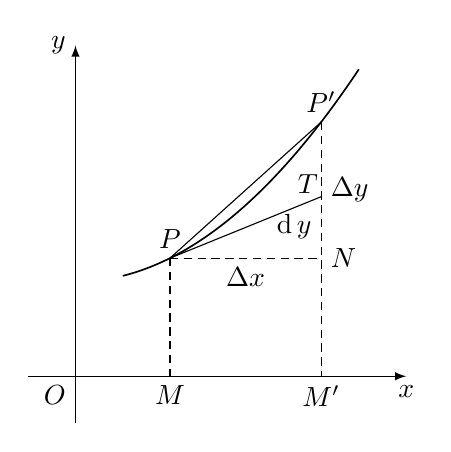
\begin{tikzpicture}[>=latex,scale=1.2]
  \draw[->](-0.5,0)--(3.5,0)node[below]{$x$};
  \draw[->](0,-0.5)--(0,3.5)node[left]{$y$};
  \node at (0,0)[below left]{$O$};
  \draw[semithick,samples=200,domain=0.5:3]plot(\x,{\x*\x*0.25+1});
  \draw[densely dashed](1,1.25)node[above]{$P$}--(1,0)node[below]{$M$};
  \draw[densely dashed](2.6,2.69)node[above]{$P'$}--(2.6,0)node[below]{$M'$};
  \draw[densely dashed](1,1.25)--(2.6,1.25)node[right]{$N$};
  \draw(1,1.25)--(2.6,2.69)(1,1.25)--(2.6,1.9)node[above left,inner sep=1pt]{$T$};
  \node at (1.8,1.25)[below]{$\Delta x$};
  \node at (2.6,1.97)[right]{$\Delta y$};
  \node at (2.6,1.58)[left]{$\mathrm{d}\,y$};
\end{tikzpicture}
\end{document}